\chapter{Kristallen II: ionaire, covalente en moleculaire vaste stoffen}\label{ch:b1:crystals-ionic-covalent}

Keukenzout breekt bij het fijnmaken in piepkleine kubusjes; diamant is het
hardste natuurlijke materiaal, en toch is grafiet, opgebouwd uit dezelfde
koolstofatomen, zacht genoeg om mee te schrijven; ijs drijft op water. Het
zijn allemaal \omterm{def:b1:crystals-metals:crystal}{kristallen}, maar hun deeltjes worden op verschillende
manieren bijeengehouden: ionen door elektrostatische aantrekking, atomen
door \omterm{def:b1:lewis-resonance-vsepr:lewis}{covalente bindingen}, moleculen door de intermoleculaire krachten van
\cref{ch:b1:intermolecular-forces-solvents}. Dit hoofdstuk past de
celgeometrie van het vorige hoofdstuk toe op deze drie families van vaste
stoffen, en verklaart uit de grootte van de ionen waarom natriumchloride
en cesiumchloride verschillende structuren aannemen.

\begin{recall}
De \omterm{def:b1:crystals-metals:multiplicity}{multipliciteit}, het \omterm{def:b1:crystals-metals:coordination}{coördinatiegetal} en de \omterm{def:b1:crystals-metals:compactness}{compactheid} van een cel,
en de octaëdrische en \omterm{def:b1:crystals-metals:site}{tetraëdrische holten} van het \omterm{def:b1:crystals-metals:packings}{kubisch
vlakgecentreerde} \omterm{def:b1:crystals-metals:lattice}{rooster}, werden gedefinieerd in
\cref{ch:b1:crystals-metals}; de dichtheid van een \omterm{def:b1:crystals-metals:crystal}{kristal} is
$\rho = ZM/(N_A V)$ (\cref{prop:b1:crystals-metals:density}). Ionstralen
werden ingevoerd in \cref{def:b1:periodicity:radius}.
\end{recall}

\section{Ionkristallen en straalverhoudingen}

\begin{definition}[Ionkristal]\label{def:b1:crystals-ionic-covalent:ionic-crystal}
Een \emph{ionkristal}\index{ionkristal} is een \omterm{def:b1:crystals-metals:crystal}{kristal} van kationen en
anionen die door elektrostatische aantrekking bijeengehouden worden. Elk
ion is omringd door ionen met een tegengestelde lading; het \omterm{def:b1:crystals-metals:crystal}{kristal} is
elektrisch neutraal, zodat de aantallen kationen en anionen in een cel in
de verhouding van de formule staan.
\end{definition}

\begin{proposition}[Eigenschappen van ionkristallen]\label{prop:b1:crystals-ionic-covalent:ionic-properties}
\omterm{def:b1:crystals-ionic-covalent:ionic-crystal}{Ionkristallen} zijn hard maar bros (een verschuiving van één laag brengt
ionen met hetzelfde teken tegenover elkaar, en het \omterm{def:b1:crystals-metals:crystal}{kristal} splijt), hebben
hoge smeltpunten, geleiden als vaste stof niet maar wel in gesmolten of
opgeloste toestand, en lossen op in \omterm{def:b1:intermolecular-forces-solvents:solvent-classes}{polaire oplosmiddelen} met een hoge
permittiviteit.
\end{proposition}
\admitted

\begin{definition}[Straalverhouding]\label{def:b1:crystals-ionic-covalent:radius-ratio}
In een \omterm{def:b1:crystals-ionic-covalent:ionic-crystal}{ionkristal} van een kation met straal $r_+$ en een anion met straal
$r_-$ is de \emph{straalverhouding}\index{straalverhouding} $x = r_+/r_-$
(meestal $x < 1$, omdat kationen kleiner zijn dan anionen).
\end{definition}

\begin{proposition}[De regel van de straalverhouding]\label{prop:b1:crystals-ionic-covalent:rule}
In het model van harde bollen is een structuur waarin elk kation $n$
anionen raakt alleen stabiel als de anionen elkaar niet raken, wat vereist
dat $x$ boven een grens ligt die door de geometrie wordt vastgelegd:
$x \ge \sqrt3 - 1
\approx 0.732$ voor 8 buren (kubus), $x \ge \sqrt2 - 1 \approx 0.414$
voor 6 (octaëder), $x \ge \sqrt{3/2} - 1 \approx 0.225$ voor 4
(tetraëder). De aangenomen structuur is die met de hoogste coördinatie
die $x$ toelaat.
\end{proposition}

\begin{proof}
Het kation zit in de holte tussen $n$ anionen waarmee het in contact is.
Aan de grens raken de anionen elkaar ook. Kubus: de anionen zitten op de
hoekpunten van een kubus met ribbe $2r_-$ en het kation in het midden,
zodat $r_+ +
r_- = \sqrt3\,r_-$. Octaëder: vier anionen in een vierkant met zijde
$2r_-$, het kation in het midden, $r_+ + r_- = \sqrt2\,r_-$. Tetraëder:
de anionen op afwisselende hoekpunten van een kubus met ribbe
$\sqrt2\,r_-$, het kation in het midden,
$r_+ + r_- = \frac{\sqrt3}{2}\sqrt2\,r_- = \sqrt{3/2}\,r_-$. Delen door
$r_-$ geeft de grenzen. Onder de grens rammelt het kation in een holte die
te groot voor hem is: de anionen stoten elkaar af zonder dat de
aantrekking toeneemt, zodat een lagere coördinatie, met een kleinere
holte, de voorkeur krijgt.
\end{proof}

\begin{omfigure}
\begin{tikzpicture}[font=\small, >={Stealth}]
  \draw[->, thick] (0,0) -- (12.4,0) node[right] {$x = r_+/r_-$};
  \foreach \x/\l in {0/0, 2.7/0.225, 4.97/0.414, 8.78/0.732, 12/1} {
    \draw (\x,0.12) -- (\x,-0.12) node[below] {\l};
  }
  \fill[omDef!15] (2.7,0.2) rectangle (4.97,1.0);
  \fill[omProp!15] (4.97,0.2) rectangle (8.78,1.0);
  \fill[omThm!15] (8.78,0.2) rectangle (12,1.0);
  \node[align=center] at (3.83,0.6) {4: ZnS};
  \node[align=center] at (6.87,0.6) {6: NaCl};
  \node[align=center] at (10.4,0.6) {8: CsCl};
  \foreach \x/\l in {3.91/\ce{ZnS}, 6.76/\ce{NaCl}, 10.08/\ce{RbCl}, 11.54/\ce{CsCl}} {
    \draw[omExo, thick] (\x,-0.55) -- (\x,-0.95);
    \node[below, omExo] at (\x,-0.95) {\l};
  }
\end{tikzpicture}

{\small De regel van de \omterm{def:b1:crystals-ionic-covalent:radius-ratio}{straalverhouding}: het \omterm{def:b1:crystals-metals:coordination}{coördinatiegetal} van het
kation dat $x$ toelaat, en de gemeten verhoudingen van vier zouten
(stralen van Shannon). Rubidiumchloride, met 0.84, zou van het
\ce{CsCl}-type moeten zijn maar neemt het \ce{NaCl}-type aan: de regel is
een leidraad, geen wet (\cref{exo:b1:crystals-ionic-covalent:12}).}
% ledger: rion:Zn2+IV, rion:S2-VI, rion:Na+VI, rion:Cl-VI, rion:Rb+VI,
% rion:Cs+VIII
\end{omfigure}


\section{Vier structuurtypen}

\begin{definition}[Structuurtypen]\label{def:b1:crystals-ionic-covalent:structure-type}
\omterm{def:b1:crystals-ionic-covalent:ionic-crystal}{Ionkristallen} worden ingedeeld in een klein aantal structuurtypen,
genoemd naar een representatieve verbinding:
\begin{itemize}
  \item \emph{cesiumchloridetype}\index{cesiumchloridetype}: anionen op de
        hoekpunten van een kubus, het kation in het midden (8:8);
  \item \emph{steenzouttype}\index{steenzouttype} (natriumchloridetype):
        anionen op een \omterm{def:b1:crystals-metals:lattice}{FCC-rooster}, kationen in al zijn \omterm{def:b1:crystals-metals:site}{octaëdrische
        holten} (6:6);
  \item \emph{zinkblendetype}\index{zinkblendetype}: anionen op een
        \omterm{def:b1:crystals-metals:lattice}{FCC-rooster}, kationen in de helft van zijn \omterm{def:b1:crystals-metals:site}{tetraëdrische holten},
        afwisselend één op twee (4:4);
  \item \emph{fluoriettype}\index{fluoriettype}: kationen op een
        \omterm{def:b1:crystals-metals:lattice}{FCC-rooster}, anionen in al zijn \omterm{def:b1:crystals-metals:site}{tetraëdrische holten} (8:4),
        formule \ce{MX2}; in het
        \emph{antifluoriettype}\index{antifluoriettype} zijn de rollen
        omgewisseld (\ce{Li2O}, 4:8).
\end{itemize}
Het getallenpaar geeft de coördinatie van het kation en van het anion.
\end{definition}

\begin{omfigure}
\tdplotsetmaincoords{60}{100}
\begin{tikzpicture}[tdplot_main_coords, font=\small]
  \pic {omcubeo={3}};
    \node[aX={green!55!black}{6.5mm}] at (0,0,0) {};
  \node[aX={violet!70}{3.8mm}] at (0,1.5,0) {};
  \node[aX={green!55!black}{6.5mm}] at (0,3,0) {};
  \node[aX={violet!70}{3.8mm}] at (0,0,1.5) {};
  \node[aX={green!55!black}{6.5mm}] at (0,1.5,1.5) {};
  \node[aX={violet!70}{3.8mm}] at (0,3,1.5) {};
  \node[aX={violet!70}{3.8mm}] at (1.5,0,0) {};
  \node[aX={green!55!black}{6.5mm}] at (0,0,3) {};
  \node[aX={green!55!black}{6.5mm}] at (1.5,1.5,0) {};
  \node[aX={violet!70}{3.8mm}] at (0,1.5,3) {};
  \node[aX={violet!70}{3.8mm}] at (1.5,3,0) {};
  \node[aX={green!55!black}{6.5mm}] at (0,3,3) {};
  \node[aX={green!55!black}{6.5mm}] at (1.5,0,1.5) {};
  \node[aX={violet!70}{3.8mm}] at (1.5,1.5,1.5) {};
  \node[aX={green!55!black}{6.5mm}] at (1.5,3,1.5) {};
  \node[aX={green!55!black}{6.5mm}] at (3,0,0) {};
  \node[aX={violet!70}{3.8mm}] at (1.5,0,3) {};
  \node[aX={violet!70}{3.8mm}] at (3,1.5,0) {};
  \node[aX={green!55!black}{6.5mm}] at (1.5,1.5,3) {};
  \node[aX={green!55!black}{6.5mm}] at (3,3,0) {};
  \node[aX={violet!70}{3.8mm}] at (1.5,3,3) {};
  \node[aX={violet!70}{3.8mm}] at (3,0,1.5) {};
  \node[aX={green!55!black}{6.5mm}] at (3,1.5,1.5) {};
  \node[aX={violet!70}{3.8mm}] at (3,3,1.5) {};
  \node[aX={green!55!black}{6.5mm}] at (3,0,3) {};
  \node[aX={violet!70}{3.8mm}] at (3,1.5,3) {};
  \node[aX={green!55!black}{6.5mm}] at (3,3,3) {};
  \node at (1.5,1.5,-1.75) {\ce{NaCl} (steenzout)};
\end{tikzpicture}
\hspace{1cm}
\begin{tikzpicture}[tdplot_main_coords, font=\small]
  \pic {omcubeo={3}};
    \node[aX={green!55!black}{6.5mm}] at (0,0,0) {};
  \node[aX={green!55!black}{6.5mm}] at (0,3,0) {};
  \node[aX={green!55!black}{6.5mm}] at (0,0,3) {};
  \node[aX={green!55!black}{6.5mm}] at (0,3,3) {};
  \node[aX={blue!60}{7mm}] at (1.5,1.5,1.5) {};
  \node[aX={green!55!black}{6.5mm}] at (3,0,0) {};
  \node[aX={green!55!black}{6.5mm}] at (3,3,0) {};
  \node[aX={green!55!black}{6.5mm}] at (3,0,3) {};
  \node[aX={green!55!black}{6.5mm}] at (3,3,3) {};
  \node at (1.5,1.5,-1.75) {\ce{CsCl}};
\end{tikzpicture}

{\small Links: de steenzoutcel, \ce{Cl-} (groen) op een \omterm{def:b1:crystals-metals:lattice}{FCC-rooster},
\ce{Na+} (violet) in elke \omterm{def:b1:crystals-metals:site}{octaëdrische holte}. Rechts: de
cesiumchloridecel, \ce{Cl-} op de hoekpunten, \ce{Cs+} (blauw) in het
midden. De ionen zijn kleiner getekend dan bij contact.}
\end{omfigure}

\begin{proposition}[Steenzout- en cesiumchloridetype]\label{prop:b1:crystals-ionic-covalent:nacl-cscl}
In het \omterm{def:b1:crystals-ionic-covalent:structure-type}{steenzouttype} is $Z = 4$ formule-eenheden per cel, raken de ionen
elkaar langs een ribbe, $a = 2(r_+ + r_-)$, en vereist de structuur
$\sqrt2 - 1
\le x$. In het \omterm{def:b1:crystals-ionic-covalent:structure-type}{cesiumchloridetype} is $Z = 1$, raken de ionen elkaar langs
de lichaamsdiagonaal, $a\sqrt3 = 2(r_+ + r_-)$, en vereist de structuur
$x \ge \sqrt3 - 1$.
\end{proposition}

\begin{proof}
Steenzout: de anionen van het \omterm{def:b1:crystals-metals:lattice}{FCC-rooster} tellen voor $4$, de kationen in
de 4 \omterm{def:b1:crystals-metals:site}{octaëdrische holten} voor $1 + 12 \times \frac14 = 4$. Langs een
ribbe volgen anion, kation en anion elkaar op in contact. De anionen
overlappen niet als de zijvlakdiagonaal, die drie anionen bevat waarvan
er hoogstens twee elkaar raken, voldoet aan $a\sqrt2 \ge 4r_-$, dus
$2(r_+ + r_-)\sqrt2 \ge
4r_-$, of $x \ge \sqrt2 - 1$. Cesiumchloride: $8 \times \frac18 = 1$
anion en 1 kation; op de lichaamsdiagonaal anion, kation, anion in
contact; de anionen overlappen niet langs een ribbe als $a \ge 2r_-$, dus
$2(r_+ + r_-)/\sqrt3 \ge 2r_-$, of $x \ge \sqrt3 - 1$.
\end{proof}

\begin{example}[Natriumchloride en cesiumchloride]\label{ex:b1:crystals-ionic-covalent:nacl}
Natriumchloride heeft $a = \qty{564.1}{pm}$: $r_+ + r_- = a/2 =
\qty{282.0}{pm}$, tegen $102 + 181 = \qty{283}{pm}$ uit de stralen van
Shannon; $x = 102/181 = 0.56$, in het octaëdrische gebied. Zijn
dichtheid is $\rho = 4 \times 58.44/(6.022 \times 10^{23} \times (5.641 \times
10^{-8})^3) = \qty{2.16}{g/cm^3}$, gemeten \qty{2.17}{g/cm^3}.
Cesiumchloride heeft $a = \qty{412.3}{pm}$: $r_+ + r_- = a\sqrt3/2 =
\qty{357.1}{pm}$, en $x = 174/181 = 0.96$, in het kubische gebied.
% ledger: lat:NaCl, rion:Na+VI, rion:Cl-VI, rho:NaCl, lat:CsCl,
% rion:Cs+VIII
\end{example}

\begin{omfigure}
\begin{minipage}[b]{0.31\linewidth}\centering
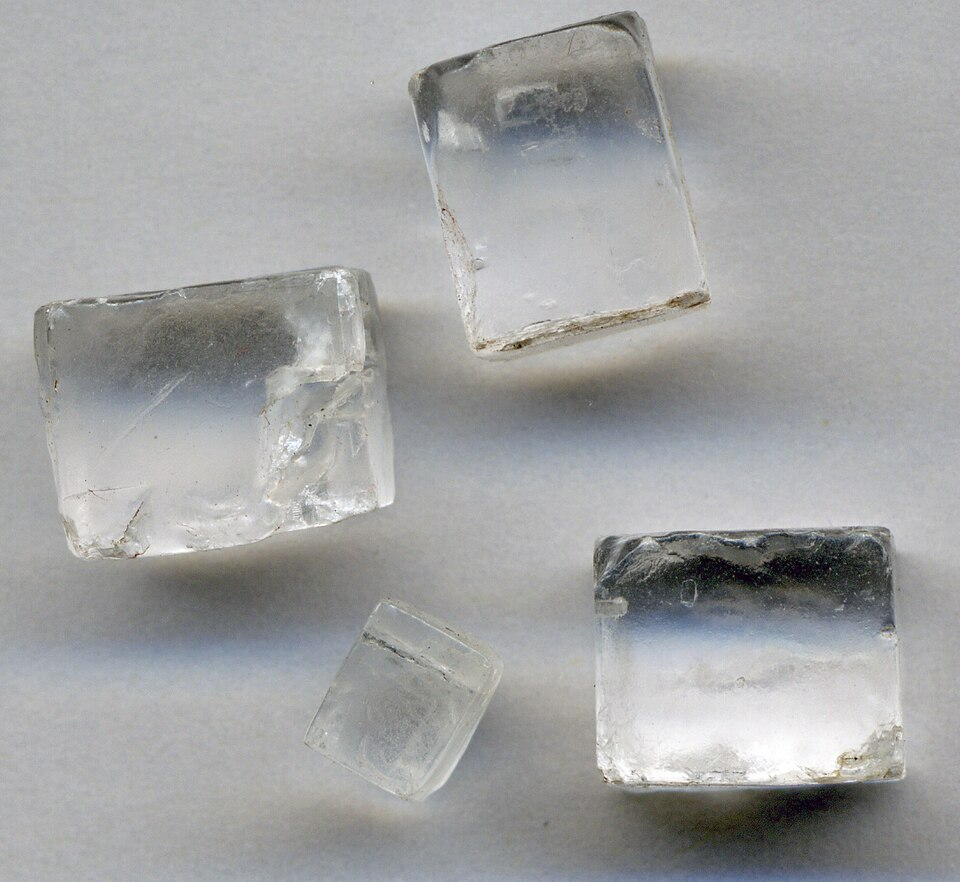
\includegraphics[width=\linewidth]{images/book2/halite.jpg}

{\small \omterm{def:b1:crystals-metals:crystal}{Kristallen} van haliet (steenzout). Foto: James St. John, CC BY 2.0.}
\end{minipage}\hfill
\begin{minipage}[b]{0.31\linewidth}\centering
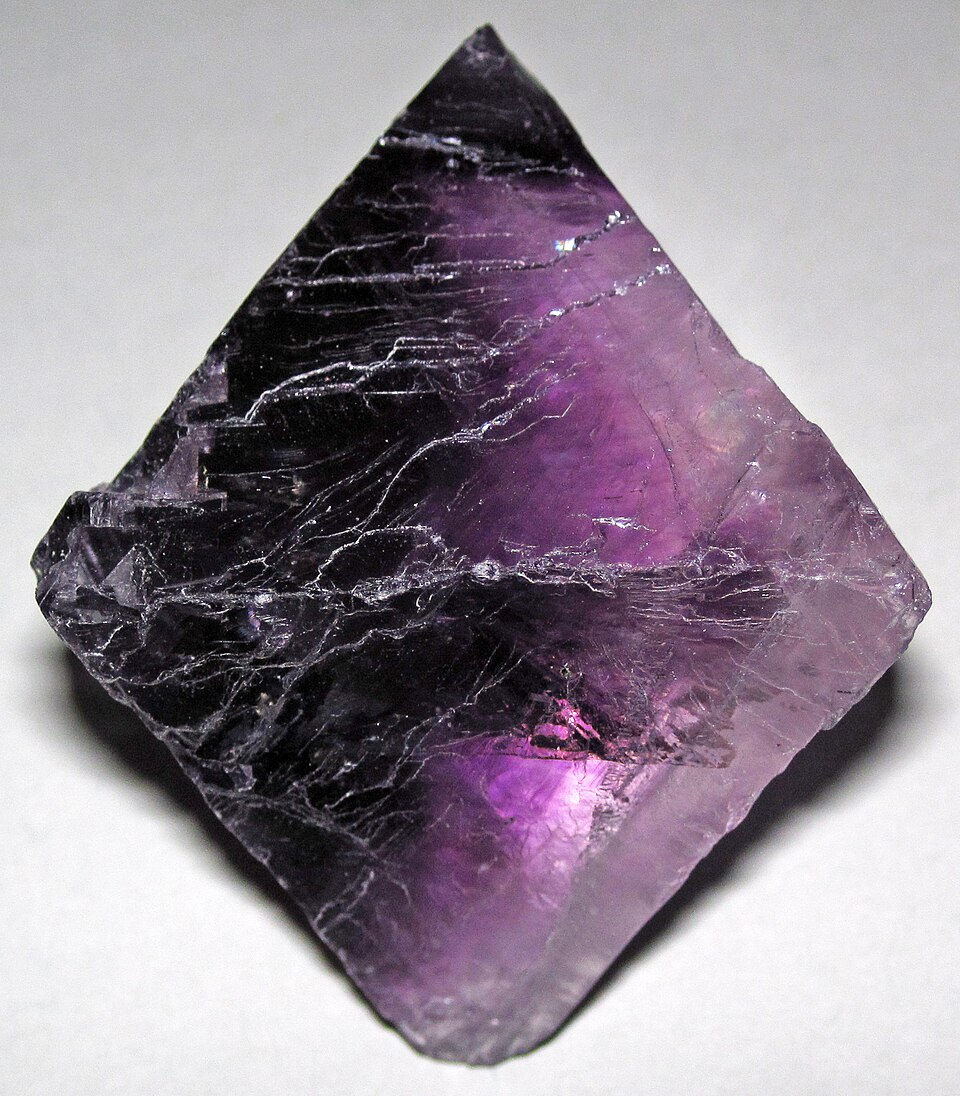
\includegraphics[width=0.85\linewidth]{images/book2/fluorite.jpg}

{\small Fluoriet, \ce{CaF2}. Foto: James St. John, CC BY 2.0.}
\end{minipage}\hfill
\begin{minipage}[b]{0.31\linewidth}\centering
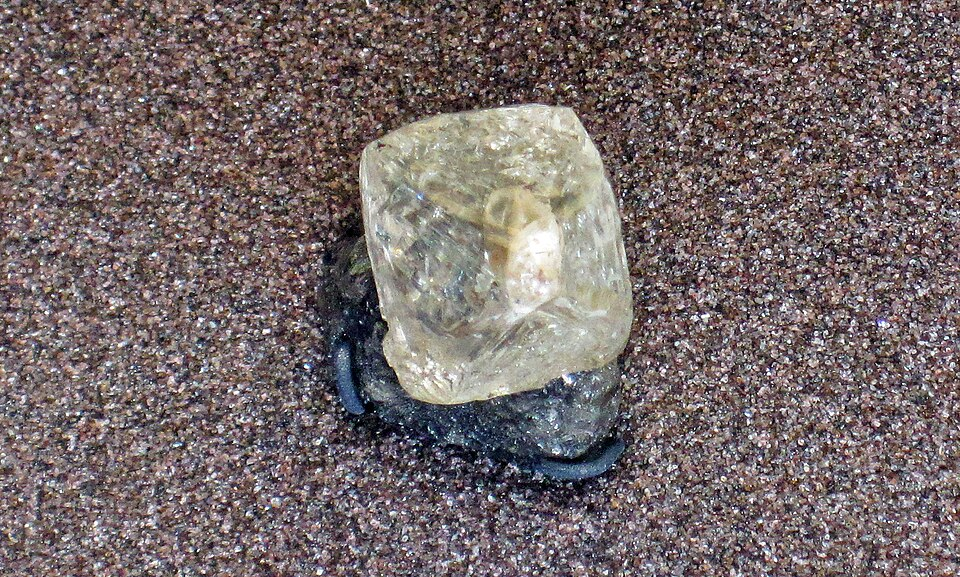
\includegraphics[width=\linewidth]{images/book2/diamond.jpg}

{\small Een ruwe diamant in de vorm van een octaëder. Foto: James St.
John, CC BY 2.0.}
\end{minipage}
\end{omfigure}

\begin{proposition}[Zinkblende- en fluoriettype]\label{prop:b1:crystals-ionic-covalent:zns-caf2}
In het \omterm{def:b1:crystals-ionic-covalent:structure-type}{zinkblendetype} is $Z = 4$, is elk ion omringd door vier ionen van
de andere soort op de hoekpunten van een tetraëder, en raken de ionen
elkaar langs een kwart van de lichaamsdiagonaal: $a\sqrt3/4 = r_+ + r_-$.
In het \omterm{def:b1:crystals-ionic-covalent:structure-type}{fluoriettype} is $Z = 4$ eenheden \ce{CaF2}, heeft elk kation 8
anionen als buren (een kubus), elk anion 4 kationen (een tetraëder), en
geldt opnieuw $a\sqrt3/4 =
r_+ + r_-$.
\end{proposition}

\begin{proof}
Zinkblende: 4 anionen op het \omterm{def:b1:crystals-metals:lattice}{FCC-rooster} en 4 kationen in de helft van de
8 \omterm{def:b1:crystals-metals:site}{tetraëdrische holten}. Een \omterm{def:b1:crystals-metals:site}{tetraëdrische holte} op
$(\frac a4,\frac a4,\frac a4)$ ligt op $\frac{a\sqrt3}{4}$ van haar vier
anionen. Fluoriet: 4 kationen en 8 anionen in alle \omterm{def:b1:crystals-metals:site}{tetraëdrische holten},
verhouding $1:2$. De 8 anionen binnen de cel vormen een kubus met ribbe
$a/2$; van de kleine kubussen van anionen bevat om de andere een kation
in het midden; een anion heeft zijn 4 naburige kationen op
$\frac{a\sqrt3}{4}$.
\end{proof}

\begin{omfigure}
\tdplotsetmaincoords{60}{100}
\begin{tikzpicture}[tdplot_main_coords, font=\small]
  \pic {omcubeo={3}};
  \begin{scope}[on background layer]
    \draw[black!45, line width=1.2pt] (0.75,0.75,2.25) -- (0,0,3) (0.75,0.75,2.25) -- (0,1.5,1.5) (0.75,0.75,2.25) -- (1.5,0,1.5) (0.75,0.75,2.25) -- (1.5,1.5,3) (0.75,2.25,0.75) -- (0,1.5,1.5) (0.75,2.25,0.75) -- (0,3,0) (0.75,2.25,0.75) -- (1.5,1.5,0) (0.75,2.25,0.75) -- (1.5,3,1.5) (2.25,0.75,0.75) -- (1.5,0,1.5) (2.25,0.75,0.75) -- (1.5,1.5,0) (2.25,0.75,0.75) -- (3,0,0) (2.25,0.75,0.75) -- (3,1.5,1.5) (2.25,2.25,2.25) -- (1.5,1.5,3) (2.25,2.25,2.25) -- (1.5,3,1.5) (2.25,2.25,2.25) -- (3,1.5,1.5) (2.25,2.25,2.25) -- (3,3,3);
  \end{scope}
    \node[aX={yellow!75!orange}{6mm}] at (0,0,0) {};
  \node[aX={yellow!75!orange}{6mm}] at (0,3,0) {};
  \node[aX={yellow!75!orange}{6mm}] at (0,1.5,1.5) {};
  \node[aX={gray!60}{3.6mm}] at (0.75,2.25,0.75) {};
  \node[aX={yellow!75!orange}{6mm}] at (0,0,3) {};
  \node[aX={yellow!75!orange}{6mm}] at (1.5,1.5,0) {};
  \node[aX={gray!60}{3.6mm}] at (0.75,0.75,2.25) {};
  \node[aX={yellow!75!orange}{6mm}] at (0,3,3) {};
  \node[aX={yellow!75!orange}{6mm}] at (1.5,0,1.5) {};
  \node[aX={gray!60}{3.6mm}] at (2.25,0.75,0.75) {};
  \node[aX={yellow!75!orange}{6mm}] at (1.5,3,1.5) {};
  \node[aX={yellow!75!orange}{6mm}] at (3,0,0) {};
  \node[aX={yellow!75!orange}{6mm}] at (1.5,1.5,3) {};
  \node[aX={yellow!75!orange}{6mm}] at (3,3,0) {};
  \node[aX={gray!60}{3.6mm}] at (2.25,2.25,2.25) {};
  \node[aX={yellow!75!orange}{6mm}] at (3,1.5,1.5) {};
  \node[aX={yellow!75!orange}{6mm}] at (3,0,3) {};
  \node[aX={yellow!75!orange}{6mm}] at (3,3,3) {};
  \node at (1.5,1.5,-1.75) {\ce{ZnS} (zinkblende)};
\end{tikzpicture}
\hspace{1cm}
\begin{tikzpicture}[tdplot_main_coords, font=\small]
  \pic {omcubeo={3}};
    \node[aX={green!35!gray}{4.4mm}] at (0,0,0) {};
  \node[aX={green!35!gray}{4.4mm}] at (0,3,0) {};
  \node[aX={green!35!gray}{4.4mm}] at (0,1.5,1.5) {};
  \node[aX={green!45!yellow}{5.0mm}] at (0.75,0.75,0.75) {};
  \node[aX={green!45!yellow}{5.0mm}] at (0.75,2.25,0.75) {};
  \node[aX={green!35!gray}{4.4mm}] at (0,0,3) {};
  \node[aX={green!35!gray}{4.4mm}] at (1.5,1.5,0) {};
  \node[aX={green!45!yellow}{5.0mm}] at (0.75,0.75,2.25) {};
  \node[aX={green!35!gray}{4.4mm}] at (0,3,3) {};
  \node[aX={green!35!gray}{4.4mm}] at (1.5,0,1.5) {};
  \node[aX={green!45!yellow}{5.0mm}] at (0.75,2.25,2.25) {};
  \node[aX={green!45!yellow}{5.0mm}] at (2.25,0.75,0.75) {};
  \node[aX={green!35!gray}{4.4mm}] at (1.5,3,1.5) {};
  \node[aX={green!35!gray}{4.4mm}] at (3,0,0) {};
  \node[aX={green!45!yellow}{5.0mm}] at (2.25,2.25,0.75) {};
  \node[aX={green!35!gray}{4.4mm}] at (1.5,1.5,3) {};
  \node[aX={green!35!gray}{4.4mm}] at (3,3,0) {};
  \node[aX={green!45!yellow}{5.0mm}] at (2.25,0.75,2.25) {};
  \node[aX={green!45!yellow}{5.0mm}] at (2.25,2.25,2.25) {};
  \node[aX={green!35!gray}{4.4mm}] at (3,1.5,1.5) {};
  \node[aX={green!35!gray}{4.4mm}] at (3,0,3) {};
  \node[aX={green!35!gray}{4.4mm}] at (3,3,3) {};
  \node at (1.5,1.5,-1.75) {\ce{CaF2} (fluoriet)};
\end{tikzpicture}

{\small Links: zinkblende, \ce{S^{2-}} (geel) op een \omterm{def:b1:crystals-metals:lattice}{FCC-rooster} en
\ce{Zn^{2+}} (grijs) in afwisselende \omterm{def:b1:crystals-metals:site}{tetraëdrische holten}, elk verbonden
met zijn vier buren. Rechts: fluoriet, \ce{Ca^{2+}} (grijsgroen) op een
\omterm{def:b1:crystals-metals:lattice}{FCC-rooster} en \ce{F-} (lichtgroen) in alle acht \omterm{def:b1:crystals-metals:site}{tetraëdrische holten}.}
\end{omfigure}

\begin{example}[Zinkblende en fluoriet]\label{ex:b1:crystals-ionic-covalent:zns}
Zinkblende heeft $a = \qty{540.9}{pm}$: $r_+ + r_- = a\sqrt3/4 =
\qty{234.2}{pm}$ (Shannon: $60 + 184 = \qty{244}{pm}$, omdat de straal
van het sulfide alleen voor zes buren getabelleerd is), en
$x = 60/184 = 0.33$, in het tetraëdrische gebied. Fluoriet heeft
$a = \qty{546.3}{pm}$: $r_+ + r_- =
\qty{236.6}{pm}$ (Shannon $112 + 131 = \qty{243}{pm}$), en $x = 0.85$:
het kation zit in een kubus van 8 anionen, zoals de regel vereist.
% ledger: lat:ZnS, rion:Zn2+IV, rion:S2-VI, lat:CaF2, rion:Ca2+VIII,
% rion:F-IV
\end{example}


\begin{method}[Een structuur voorspellen]\label{met:b1:crystals-ionic-covalent:predict}
Zo voorspel je de structuur van een ionaire verbinding \ce{MX} of
\ce{MX2}:
\begin{enumerate}
  \item bereken $x = r_+/r_-$ uit getabelleerde stralen (voor de
        verwachte coördinatie);
  \item lees de coördinatie van het kation af uit de regel van de
        \omterm{def:b1:crystals-ionic-covalent:radius-ratio}{straalverhouding};
  \item kies het type met die coördinatie en de juiste formule:
        \ce{MX} met 8: \ce{CsCl}; met 6: \ce{NaCl}; met 4: zinkblende;
        \ce{MX2} met 8: fluoriet;
  \item controleer met de gemeten roosterparameter; bedenk dat
        polariseerbare ionen (\ce{S^{2-}}, \ce{I-}) en kleine, geladen
        kationen deels \omterm{def:b1:lewis-resonance-vsepr:lewis}{covalente bindingen} geven, waarvoor de regel
        faalt.
\end{enumerate}
\end{method}

\section{Covalente kristallen}

\begin{definition}[Covalent kristal]\label{def:b1:crystals-ionic-covalent:covalent-crystal}
Een \emph{covalent kristal}\index{covalent kristal} (of netwerkvaste
stof) is een \omterm{def:b1:crystals-metals:crystal}{kristal} waarin alle atomen door \omterm{def:b1:lewis-resonance-vsepr:lewis}{covalente bindingen} tot één
reuzenmolecuul verbonden zijn: diamant, silicium, kwarts \ce{SiO2}. In een
gelaagd covalent \omterm{def:b1:crystals-metals:crystal}{kristal} zoals grafiet strekt het covalente netwerk zich
alleen in vlakken uit, die door \omterm{def:b1:intermolecular-forces-solvents:vdw}{vanderwaalsinteracties} aan elkaar
gehouden worden.
\end{definition}

\begin{proposition}[De diamantstructuur]\label{prop:b1:crystals-ionic-covalent:diamond}
In diamant bezetten de koolstofatomen het \omterm{def:b1:crystals-metals:lattice}{FCC-rooster} en de helft van zijn
\omterm{def:b1:crystals-metals:site}{tetraëdrische holten}, zoals de twee soorten ionen van zinkblende:
$Z = 8$, elk koolstofatoom gebonden aan vier andere op de hoekpunten van
een tetraëder, op de afstand $a\sqrt3/4$. Voor bollen die elkaar raken,
is de \omterm{def:b1:crystals-metals:compactness}{compactheid}
\[
  C = \frac{\pi\sqrt3}{16} \approx 0.34 .
\]
\end{proposition}


\begin{proof}
$Z = 4 + 4 = 8$. Naburige atomen raken elkaar: $2R = a\sqrt3/4$, dus $a =
8R/\sqrt3$ en $C = 8 \cdot \frac43\pi R^3/a^3 = \frac{32}{3}\pi R^3 \cdot
\frac{3\sqrt3}{512 R^3} = \frac{\pi\sqrt3}{16}$.
\end{proof}

\begin{omfigure}
\tdplotsetmaincoords{60}{100}
\begin{tikzpicture}[tdplot_main_coords, font=\small]
  \pic {omcubeo={3}};
  \begin{scope}[on background layer]
    \draw[black!55, line width=1.4pt] (0.75,0.75,2.25) -- (0,0,3) (0.75,0.75,2.25) -- (0,1.5,1.5) (0.75,0.75,2.25) -- (1.5,0,1.5) (0.75,0.75,2.25) -- (1.5,1.5,3) (0.75,2.25,0.75) -- (0,1.5,1.5) (0.75,2.25,0.75) -- (0,3,0) (0.75,2.25,0.75) -- (1.5,1.5,0) (0.75,2.25,0.75) -- (1.5,3,1.5) (2.25,0.75,0.75) -- (1.5,0,1.5) (2.25,0.75,0.75) -- (1.5,1.5,0) (2.25,0.75,0.75) -- (3,0,0) (2.25,0.75,0.75) -- (3,1.5,1.5) (2.25,2.25,2.25) -- (1.5,1.5,3) (2.25,2.25,2.25) -- (1.5,3,1.5) (2.25,2.25,2.25) -- (3,1.5,1.5) (2.25,2.25,2.25) -- (3,3,3);
  \end{scope}
  \node[aX={black!65}{3.6mm}] at (0,0,0) {};
  \node[aX={black!65}{3.6mm}] at (0,3,0) {};
  \node[aX={black!65}{3.6mm}] at (0,1.5,1.5) {};
  \node[aX={black!65}{3.6mm}] at (0.75,2.25,0.75) {};
  \node[aX={black!65}{3.6mm}] at (0,0,3) {};
  \node[aX={black!65}{3.6mm}] at (1.5,1.5,0) {};
  \node[aX={black!65}{3.6mm}] at (0.75,0.75,2.25) {};
  \node[aX={black!65}{3.6mm}] at (0,3,3) {};
  \node[aX={black!65}{3.6mm}] at (1.5,0,1.5) {};
  \node[aX={black!65}{3.6mm}] at (2.25,0.75,0.75) {};
  \node[aX={black!65}{3.6mm}] at (1.5,3,1.5) {};
  \node[aX={black!65}{3.6mm}] at (3,0,0) {};
  \node[aX={black!65}{3.6mm}] at (1.5,1.5,3) {};
  \node[aX={black!65}{3.6mm}] at (3,3,0) {};
  \node[aX={black!65}{3.6mm}] at (2.25,2.25,2.25) {};
  \node[aX={black!65}{3.6mm}] at (3,1.5,1.5) {};
  \node[aX={black!65}{3.6mm}] at (3,0,3) {};
  \node[aX={black!65}{3.6mm}] at (3,3,3) {};
  \node at (1.5,1.5,-1.75) {diamant};
\end{tikzpicture}
\hspace{0.8cm}
\begin{tikzpicture}[font=\small, y={(0cm,0.45cm)}, z={(0cm,1cm)}, x={(1cm,0cm)}]
  % two honeycomb layers seen in perspective, ABAB stacking
  \foreach \zz/\dy/\col in {0/0/black!40, 1.7/0.82/black!80} {
    \foreach \i in {0,1,2} \foreach \j in {0,1} {
      \pgfmathsetmacro\cx{1.42*\i+0.71*\j}
      \pgfmathsetmacro\cy{1.23*\j+\dy}
      \foreach \k in {0,60,...,300} {
        \pgfmathsetmacro\ka{\k+60}
        \draw[\col, line width=1pt] ({\cx+0.82*cos(\k+30)},{\cy+0.82*sin(\k+30)},\zz)
          -- ({\cx+0.82*cos(\ka+30)},{\cy+0.82*sin(\ka+30)},\zz);
      }
    }
  }
  \draw[<->, omThm] (5.6,0.9,0) -- (5.6,0.9,1.7) node[midway, right] {\qty{335}{pm}};
  \node at (2.4,-1.6,0) {grafiet};
\end{tikzpicture}

{\small Links: de diamantcel, elk koolstofatoom gebonden aan vier andere
in een tetraëder. Rechts: grafiet, lagen van zeshoeken (C--C
\qty{141.8}{pm} binnen een laag) gestapeld op \qty{334.8}{pm} van
elkaar, bijeengehouden door londonkrachten; de lagen wisselen af
volgens ABAB.}
% ledger: lat:C-graphite.a, lat:C-graphite.c (C-C = a/sqrt3; interlayer = c/2)
\end{omfigure}


\begin{example}[Diamant, silicium, grafiet]\label{ex:b1:crystals-ionic-covalent:carbon}
Diamant heeft $a = \qty{356.7}{pm}$: \ce{C-C} $= a\sqrt3/4 =
\qty{154.5}{pm}$, de enkele binding van ethaan, en $\rho =
\qty{3.52}{g/cm^3}$. Silicium, met dezelfde structuur en $a =
\qty{543.1}{pm}$, heeft \ce{Si-Si} $= \qty{235.2}{pm}$ en $\rho =
\qty{2.33}{g/cm^3}$ (gemeten 2.33). In grafiet is elk koolstofatoom in
een vlak gebonden aan drie andere op \qty{141.8}{pm}, een bindingsorde
tussen één en twee (resonantie over de laag), terwijl de lagen
\qty{334.8}{pm} uit elkaar liggen. Diamant, star in drie dimensies, is
het hardste natuurlijke materiaal en een isolator; grafiet splijt tussen
zijn lagen, die gemakkelijk over elkaar glijden, en geleidt elektriciteit
binnen de lagen dankzij zijn gedelokaliseerde $\pi$-elektronen.
% ledger: lat:C-diamond, lat:Si, rho:Si, lat:C-graphite.a, lat:C-graphite.c,
% geo:C2H6.rCC
\end{example}

\begin{omfigure}
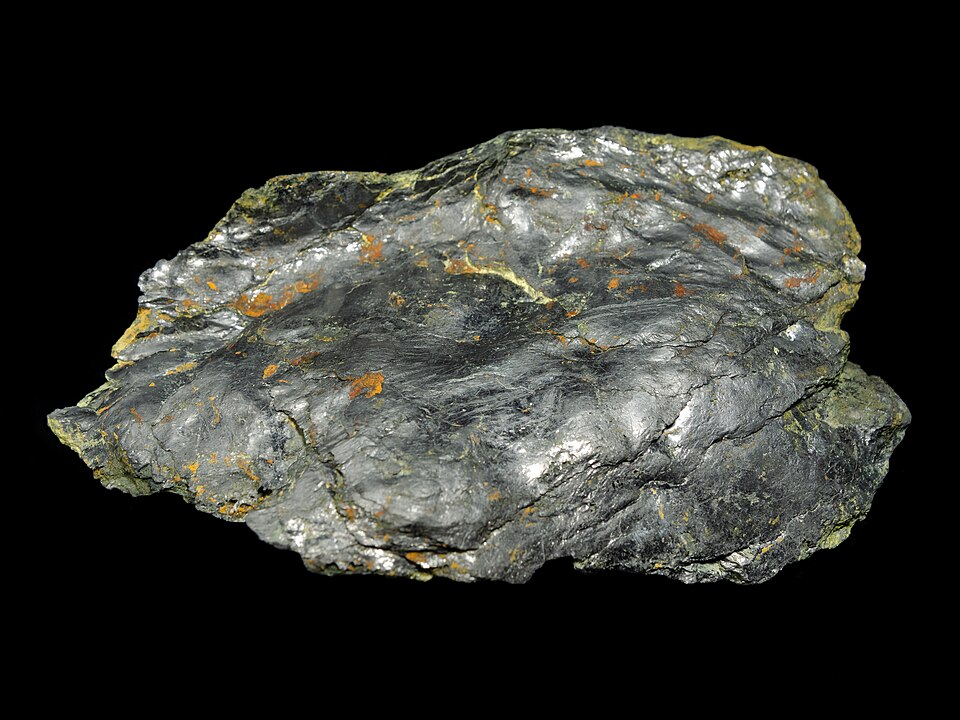
\includegraphics[width=0.36\linewidth]{images/book2/graphite.jpg}

{\small Een stuk natuurlijk grafiet, met zijn metaalglans. Foto:
Zbynek Burival, CC BY-SA 4.0.}
\end{omfigure}

\section{Moleculaire kristallen}

\begin{definition}[Moleculair kristal]\label{def:b1:crystals-ionic-covalent:molecular-crystal}
Een \emph{moleculair kristal}\index{moleculair kristal} is een \omterm{def:b1:crystals-metals:crystal}{kristal} van
moleculen die door intermoleculaire krachten bijeengehouden worden ---
\omterm{def:b1:intermolecular-forces-solvents:vdw}{vanderwaalsinteracties} en, als dat kan, \omterm{def:b1:intermolecular-forces-solvents:hbond}{waterstofbruggen} ---, terwijl elk
molecuul zijn eigen \omterm{def:b1:lewis-resonance-vsepr:lewis}{covalente bindingen} behoudt: dijood, droogijs
\ce{CO2(s)}, ijs, suiker.
\end{definition}

\begin{proposition}[Eigenschappen van moleculaire kristallen]\label{prop:b1:crystals-ionic-covalent:molecular}
\omterm{def:b1:crystals-ionic-covalent:molecular-crystal}{Moleculaire kristallen} zijn zacht en smelten of sublimeren bij lage
temperaturen, omdat alleen zwakke intermoleculaire krachten verbroken
worden; ze geleiden niet.
\end{proposition}
\admitted

\begin{example}[IJs]\label{ex:b1:crystals-ionic-covalent:ice}
In gewoon ijs is elk watermolecuul via \omterm{def:b1:intermolecular-forces-solvents:hbond}{waterstofbruggen} gebonden aan vier
andere op de hoekpunten van een tetraëder: twee via zijn eigen
waterstofatomen en twee via zijn \omterm{def:b1:lewis-resonance-vsepr:lewis}{vrije paren}. Dit open, hexagonale
netwerk, opgelegd door de richtingen van de \omterm{def:b1:intermolecular-forces-solvents:hbond}{waterstofbruggen}, laat veel
lege ruimte: ijs is minder dicht dan vloeibaar water, waarin het netwerk
gedeeltelijk verbroken is en de moleculen dichter bij elkaar komen. De
hexagonale symmetrie van het netwerk is te zien in de zesvoudige vorm van
sneeuwkristallen.
\end{example}

\begin{omfigure}
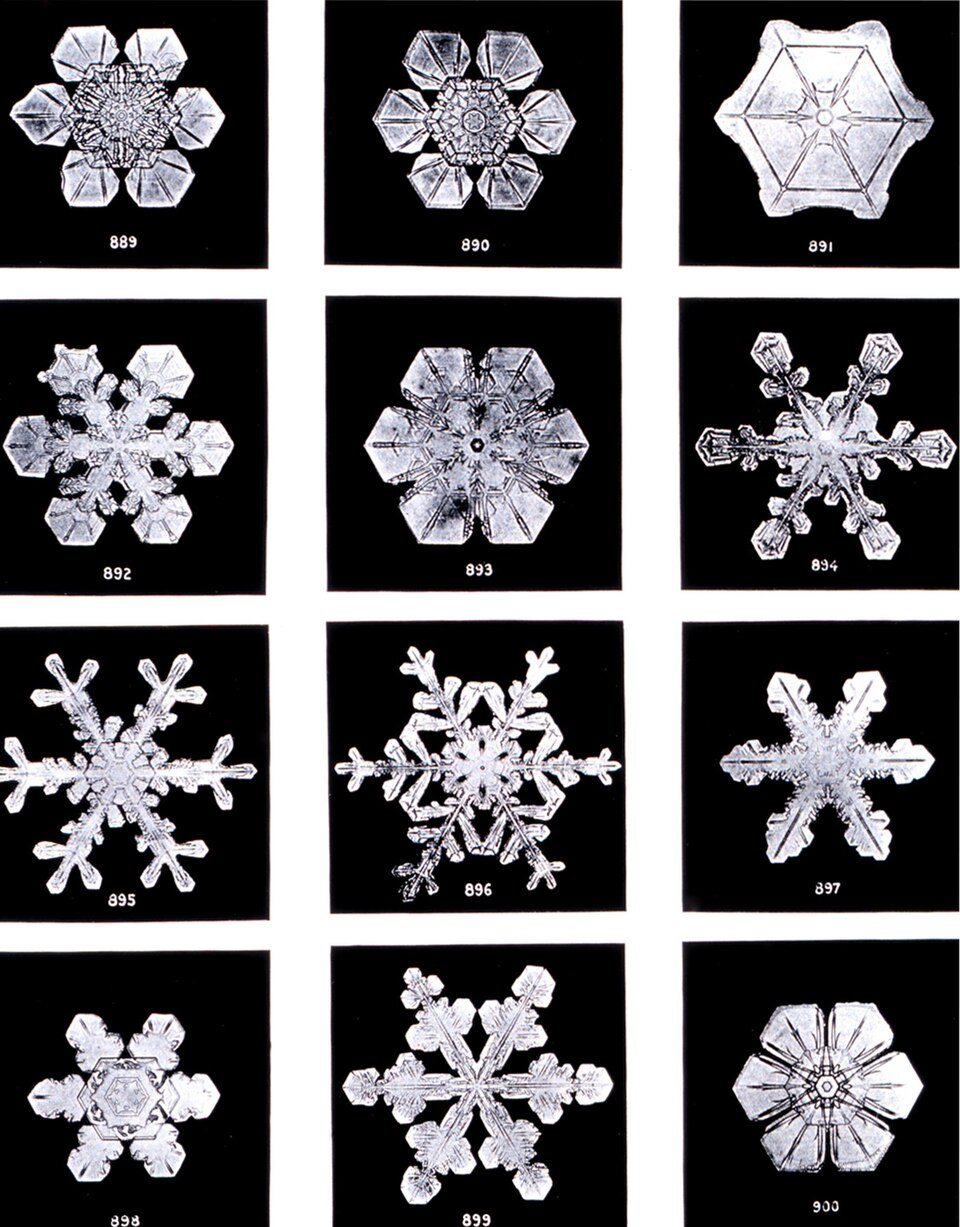
\includegraphics[width=0.38\linewidth]{images/book2/bentley-snowflakes.jpg}

{\small Sneeuwkristallen, gefotografeerd door Wilson Bentley omstreeks
1902: elk ervan heeft een zesvoudige symmetrie, het spoor van het
hexagonale netwerk van \omterm{def:b1:intermolecular-forces-solvents:hbond}{waterstofbruggen} in ijs. Publiek domein.}
\end{omfigure}

\section{De vier soorten vaste stoffen vergeleken}

\begin{center}
\small
\begin{tabular}{lllll}
\hline
vaste stof & deeltjes & cohesie & eigenschappen & voorbeelden \\
\hline
metallisch & kationen, elektronen & \omterm{def:b1:crystals-metals:metallic-bond}{metaalbinding} & geleider, taai & \ce{Cu}, \ce{Fe}, \ce{Na} \\
ionair & kationen, anionen & elektrostatisch & hard, bros, isolerend & \ce{NaCl}, \ce{CaF2} \\
covalent & atomen & \omterm{def:b1:lewis-resonance-vsepr:lewis}{covalente bindingen} & zeer hard, hoogsmeltend & diamant, \ce{SiO2} \\
moleculair & moleculen & vanderwaals, H-bruggen & zacht, laagsmeltend & \ce{I2}, ijs \\
\hline
\end{tabular}
\end{center}


\begin{remark}[Een continuüm]\label{rem:b1:crystals-ionic-covalent:continuum}
De klassen zijn idealiseringen. Zinksulfide heeft bindingen die deels
ionair en deels covalent zijn, en daarom is de afstand tussen sulfide en
zink kleiner dan de som van de ionstralen; grafiet is covalent binnen
zijn lagen en moleculair ertussen. Het verschil in \omterm{def:b1:periodicity:electronegativity}{elektronegativiteit}
(\cref{prop:b1:periodicity:en-trend}) is de leidraad: hoe groter het is,
hoe ionairder de vaste stof.
\end{remark}

\section{Oefeningen}

\begin{exercise}[$\star$]\label{exo:b1:crystals-ionic-covalent:1}
Tel in de steenzoutcel de kationen en de anionen, geef de coördinatie
van elk, en controleer dat de formule \ce{NaCl} gerespecteerd wordt.
\end{exercise}

\begin{exercise}[$\star$]\label{exo:b1:crystals-ionic-covalent:2}
Cesiumchloride heeft $a = \qty{412.3}{pm}$. Bereken de kortste
\ce{Cs-Cl}-afstand en het aantal formule-eenheden per cel.
\end{exercise}

\begin{exercise}[$\star$]\label{exo:b1:crystals-ionic-covalent:3}
Bereken met de stralen $r(\ce{Na+}) = \qty{102}{pm}$ en $r(\ce{Cl-}) =
\qty{181}{pm}$ de \omterm{def:b1:crystals-ionic-covalent:radius-ratio}{straalverhouding} van \ce{NaCl} en voorspel de
coördinatie van het kation.
\end{exercise}

\begin{exercise}[$\star$]\label{exo:b1:crystals-ionic-covalent:4}
Deel in als metallisch, ionair, covalent of moleculair: koper,
natriumchloride, diamant, dijood, kwarts \ce{SiO2}, ijs, calciumfluoride.
\end{exercise}

\begin{exercise}[$\star\star$]\label{exo:b1:crystals-ionic-covalent:5}
Bewijs dat de steenzoutstructuur $r_+/r_- \ge \sqrt2 - 1$ vereist.
\end{exercise}

\begin{exercise}[$\star\star$]\label{exo:b1:crystals-ionic-covalent:6}
Bereken de dichtheid van natriumchloride uit $a = \qty{564.1}{pm}$
($M(\ce{NaCl}) = \qty{58.44}{g/mol}$) en vergelijk met
\qty{2.17}{g/cm^3}.
\end{exercise}

\begin{exercise}[$\star\star$]\label{exo:b1:crystals-ionic-covalent:7}
Bereken de dichtheid van cesiumchloride ($M = \qty{168.36}{g/mol}$,
$a = \qty{412.3}{pm}$) en vergelijk met de gemeten \qty{3.99}{g/cm^3}.
% ledger: rho:CsCl
\end{exercise}


\begin{exercise}[$\star\star$]\label{exo:b1:crystals-ionic-covalent:8}
Bereken voor zinkblende ($a = \qty{540.9}{pm}$, $M = \qty{97.44}{g/mol}$)
de \ce{Zn-S}-afstand en de dichtheid, en vergelijk met de gemeten
\qty{4.04}{g/cm^3}.
% ledger: rho:ZnS
\end{exercise}


\begin{exercise}[$\star\star$]\label{exo:b1:crystals-ionic-covalent:9}
Grafiet heeft een hexagonale cel met $a = \qty{245.6}{pm}$ en
$c = \qty{669.6}{pm}$, die 4 atomen bevat. Bereken de \ce{C-C}-afstand
binnen een laag ($a/\sqrt3$), de afstand tussen de lagen ($c/2$) en de
dichtheid. Waarom is grafiet minder dicht dan diamant?
\end{exercise}

\begin{exercise}[$\star\star\star$]\label{exo:b1:crystals-ionic-covalent:10}
Bewijs dat de \omterm{def:b1:crystals-metals:compactness}{compactheid} van diamant $\pi\sqrt3/16$ is, en leg uit
waarom het hardste materiaal een van de minst compacte is.
\end{exercise}

\begin{exercise}[$\star\star\star$]\label{exo:b1:crystals-ionic-covalent:11}
Silicium heeft de diamantstructuur met $a = \qty{543.1}{pm}$. Bereken de
lengte van de \ce{Si-Si}-binding, de \omterm{def:b1:periodicity:radius}{covalente straal} van silicium en de
dichtheid ($M = \qty{28.09}{g/mol}$); vergelijk met \qty{2.33}{g/cm^3}.
\end{exercise}

\begin{exercise}[$\star\star\star$]\label{exo:b1:crystals-ionic-covalent:12}
Voor rubidiumchloride is $r(\ce{Rb+}) = \qty{152}{pm}$ (zes buren) en
$r(\ce{Cl-}) = \qty{181}{pm}$. Welke structuur voorspelt de regel van de
\omterm{def:b1:crystals-ionic-covalent:radius-ratio}{straalverhouding}? Onder gewone omstandigheden is het van het \omterm{def:b1:crystals-ionic-covalent:structure-type}{steenzouttype}
met $a = \qty{658.1}{pm}$: controleer de \ce{Rb-Cl}-afstand, en geef een
mogelijke reden waarom de regel hier faalt.
% ledger: rion:Rb+VI, rion:Cl-VI, lat:RbCl
\end{exercise}


\section{Probleem: fluoriet, het mineraal en de lens}

\begin{problem}[{Weekendprobleem --- de fluorietcel, haar \omterm{def:b1:crystals-ionic-covalent:radius-ratio}{straalverhouding},
twee verwanten (\ce{Li2O} en diamant), en de dichtheid van fluoriet
berekend uit zijn cel}]
\label{pb:b1:crystals-ionic-covalent:1}
Fluoriet, \ce{CaF2}, is een mineraal; als grote heldere \omterm{def:b1:crystals-metals:crystal}{kristallen} gekweekt
levert het lenzen die ultraviolet licht doorlaten. Zijn cel is kubisch,
$a =
\qty{546.3}{pm}$; \ce{Ca^{2+}} op een \omterm{def:b1:crystals-metals:lattice}{FCC-rooster}, \ce{F-} in de
\omterm{def:b1:crystals-metals:site}{tetraëdrische holten}. Stralen: $r(\ce{Ca^{2+}}) = \qty{112}{pm}$ (acht
buren), $r(\ce{F-}) = \qty{131}{pm}$ (vier buren). Molaire massa's
(g/mol): \ce{Ca} 40.08, \ce{F} 19.00, \ce{Li} 6.94, \ce{O} 16.00, \ce{C}
12.01, \ce{Si} 28.09; $N_A = \qty{6.022e23}{mol^{-1}}$.
% ledger: lat:CaF2, rion:Ca2+VIII, rion:F-IV, aw:Ca, aw:F, aw:Li, aw:O,
% aw:C, aw:Si, const:NA

\medskip
\noindent\textbf{Deel I --- De cel.}
\begin{enumerate}
  \item Geef de posities van de \ce{Ca^{2+}}-ionen in de cel en tel ze.
  \item Hoeveel \omterm{def:b1:crystals-metals:site}{tetraëdrische holten} bevat de cel? Leid het aantal
        \ce{F-}-ionen af en controleer de formule.
  \item Wat is de coördinatie van \ce{F-}? En van \ce{Ca^{2+}}?
  \item Bereken de kortste \ce{Ca-F}-afstand.
  \item Vergelijk die met de som van de ionstralen.
  \item Bereken de kortste \ce{F-F}-afstand en zeg of de anionen elkaar
        raken.
\end{enumerate}

\medskip
\noindent\textbf{Deel II --- De \omterm{def:b1:crystals-ionic-covalent:radius-ratio}{straalverhouding}.}
\begin{enumerate}[resume]
  \item Bereken $x = r_+/r_-$.
  \item Welke coördinatie van het kation laat de regel van de
        \omterm{def:b1:crystals-ionic-covalent:radius-ratio}{straalverhouding} toe?
  \item Waarom kan \ce{CaF2} de cesiumchloridestructuur niet aannemen,
        hoewel zijn kation een coördinatie 8 heeft?
  \item Beschrijf fluoriet als een enkelvoudig kubische schikking van
        \ce{F-} met \ce{Ca^{2+}} in het midden van de helft van de kleine
        kubussen.
  \item Bereken de \omterm{def:b1:crystals-metals:compactness}{compactheid} van fluoriet.
\end{enumerate}

\medskip
\noindent\textbf{Deel III --- Twee verwanten.}
Lithiumoxide, \ce{Li2O}, is antifluoriet met $a = \qty{461.9}{pm}$;
$r(\ce{Li+}) = \qty{59}{pm}$ (vier buren), $r(\ce{O^{2-}}) =
\qty{142}{pm}$ (acht buren). Diamant: $a = \qty{356.7}{pm}$.
% ledger: lat:Li2O, rion:Li+IV, rion:O2-VIII, rho:Li2O, lat:C-diamond
\begin{enumerate}[resume]
  \item Waar zitten de \ce{O^{2-}}- en de \ce{Li+}-ionen in de
        antifluorietcel?
  \item Bereken de \ce{Li-O}-afstand en vergelijk met de som van de
        stralen.
  \item Bereken de dichtheid van \ce{Li2O} en vergelijk met de gemeten
        \qty{2.01}{g/cm^3}.
  \item Welke ionaire structuur heeft dezelfde schikking van posities als
        diamant?
  \item Bereken de lengte van de \ce{C-C}-binding en de dichtheid van
        diamant.
  \item Waarom is diamant zoveel minder compact dan fluoriet, hoewel zijn
        atomen hetzelfde soort posities innemen?
\end{enumerate}

\medskip
\noindent\textbf{Deel IV --- De dichtheid van fluoriet.}
\begin{enumerate}[resume]
  \item Bereken de molaire massa van \ce{CaF2}.
  \item Bereken de massa van één cel.
  \item Bereken het volume van één cel, in \unit{cm^3}.
  \item Wat zou een vacature op één \ce{F-}-plaats per honderd cellen met
        de dichtheid doen?
  \item Bereken de dichtheid van fluoriet uit zijn cel, en vergelijk met de
        gemeten \qty{3.18}{g/cm^3}.
\end{enumerate}
% ledger: rho:CaF2
\end{problem}
